
a)texture in scene images
texture 
In computer graphics,  
texture mapping is a powerful tool which adds the surface detail to an object by wrapping
the color information from a digitized image. 
Texture is applied on top of a
polygon or 3D model to obtain a realistic rendering of it.
This makes rendering of objects more realistic than those without
surface texture. 

There are several texture mapping methods that avoids
modeling of the complex surface details. 
Images are extensively
used as source of textures as they are able to capture visual and structural information of the real world. They
are also capture a high level detail of object properties.
Generally an image is used as a texture map
on a planar surface. However this method fails if the lighting conditions of the synthetic
environment are different from the lighting conditions of the texture image. To solve this
problem, people have used image based modeling and rendering (IBMR) techniques. In these meth-
ods several images of the same object are taken under varying lighting directions with a fixed
viewpoint. These methods construct a surface reflectance model which characterizes surface
appearance under different lighting directions. fgf

3D textures are a way to model the relation between surface reflectance
properties and illumination/viewing conditions. The use of 3D texture modeling
results in enhanced realism of the scene. Reflectance texture maps are one of
the techniques that can be used to compactly represent the 3D textures. Theseml
maps are generated using image re-lighting techniques in which
multiple images are captured under different lighting/viewing conditions.

% Bidirectional Reflectance Distribution Function, which defines the
% spectral and reflectance characteristics of a surface can be used to create
% reflectance texture maps. It is defined as the ratio of reflected radiance to
% incident irradiance, given the lighting and viewing directions. The reflectance
% at each point on a surface is hence a function of four parameters, controlling
% the above two directions. Various techniques have been developed to compactly
% represent BRDF. It was extended to Bidirectional
% Texture Function by allowing BRDF to vary spatially across planar
% texture co-ordinate (u,v).

% (commented) 3D Texture modelling is an important area in computer graphics as it results in realistic rendering
% of natural material surfaces.The characterization of surface reflectance properties is important in
% achieving photorealism.The appearance of a surface in different lighting and viewing direction/
% conditions is affected by its reflectance properties.3D texture actually models the relation
% between surface reflectance properties and illumination direction. They are represented
% by Reflectance Texture Maps.These maps are generated using image re-lighting techniques
% which model the surface reflectance properties of object.
% 
% 2D texture modelling fails to capture the surface variation and reflectance properties under
% varying lighting and viewing direction.They appear good only when viewed from similar lighting
% direction in which they were captured.2D textures appear flat and smooth but reflectance properties
% of real world objects are characterised by inter-reflections,shadows,specularity and sub-surface
% scattering. 2D texture fails to provide the information required for rendering other than the original
% illumination condition. Figure 1 illustrates how  the same texture behaves differently under different lighting conditions.
% 
% It is clear from thefigure that 2D texture which has only the color information alone is not sufficient for a realisitic
%  rendering of real world texture
% and therefore 3D texture is needed.

% Reflectance map required in 3D texture can be modelled by Bidirectional Reflectance Distribution
% Function \cite{B1} technique which defines spectral and spatial reflectance characteristic of a
% surface.BRDF is the ratio of reflected radiance to incident irradiance.Various techniques have been
% developed to compactly represent BRDF \cite{B5,B8,B12,B14,B15}.
% 
% BRDF was extended to Bidirectional Texture Function \cite{B2} by allowing BRDF to vary spatially
% across planar texture co-ordinate (u,v)
% 
% (uncomment)
% \begin{math}
% $\[BTF=(\theta_{v},\phi_{v},\theta_{e},\phi_{e},u,v)\]$
% \end{math}


% BTF effectively captures view point dependent phenomenon such as specularity
% along with other physical phenomenon such as shadow, sub-surface scattering,
% inter-reflection, etc. However, the capture of BTF requires careful camera
% calibration and capturing numerous images for sampling. Generating reflectance
% map from BTF is very complex. View dependent appearances can also be modeled
% using Light field maps. They offer a more compact representation and
% can be used for a real time rendering of surface light fields.
% 
% Because of the  high dimensionality of the BTF and high storage requirement,
% Unidirectional Texture Functions (UTF) were introduced in which viewing point is
% not taken into account while modeling the surface reflectance properties. They
% model these properties only in relation to different lighting conditions. As the
% visual appearance of the surface is mostly independent of the viewing direction,
% the model provides a reasonable approximation of the surface with significantly
% lower complexity of the model.
% 
% Polynomial Texture Maps belong to the class of UTFs. It is a pixel
% based technique that concisely models the surface reflectance properties using a
% polynomial model for the reflectance, dependent on two angular parameters of the
% lighting direction. PTMs reconstruct the color of the surface under varying
% lighting conditions and models real world phenomenon such as
% self-shadowing,inter-reflection and sub-surface scattering. They thus introduce
% enhanced photorealism in the texture mapping process.
\section{Image Based Rendering}
To be written.

Image-based rendering techniques are widely used in computer graphics.
Most frequently image-based rendering appears in the form of texture mapping 
when an image is used to represent a complex object's 
appearance. Texture mapping has several significant limitations, the primary one being that only a single lighting 
condition is captured. If dynamic lighting is needed, texture mapping alone is insufficient. 

% Texture mapping is also an image-based rendering technique where images are used in place of complex geometry and material 
% properties. However, if realistic renderings are a primary
% objective, then beginning with photographs is quick and straightforward way to achieve photorealism. By starting
% with a photograph from the real world it is possible to capture complex light interactions such as interreflections,
% self shadowing, and subsurface scattering without modeling and simulation.
% Perhaps the main disadvantage of using a photograph as your rendering source is that the photograph captures the
% appearance of your object from a single viewpoint, under a static lighting condition, at a single point in time. If
% the desired rendered environment in your game does not exactly match the acquired conditions then your texture 
% will not appear realistic. While you may be able closely match the in game environment with your source 
% environment, you probably want a dynamically changing scene, where the lighting can vary, as well as the user's
% viewpoint. For an image-based technique to be dynamic a single static image is obviously insufficient.

\section{Bump Mapping}
To be written
% Bump mapping, normal mapping, and other related techniques have been developed to extend texture mapping to
% reproduce such light and view dependent dynamic effects. As with texture mapping, these methods store spatially
% variant information for rendering. However, instead of storing a texture image that already contains some existing
% illumination effects as in typical texture mapping, these methods store parameters that allow a computational 
% lighting model to be varied spatially. Since these methods are often used with simple synthetic reflectance models
% such as Phong lighting they achieve dynamic illumination at the expense of photorealism.
% Bump maps and other similar methods typically use a map that has been generated by an artist or a procedural
% method, rather than one captured from real world objects. Creating a bump map from photographs of real objects
% is difficult, and is generally not done for games or other realistic renderings. Research techniques have been
% developed to calculate bump maps automatically from multiple images of an object under known light directions 
% [Rushmeier 97]. Unfortunately these methods typically have difficulty generating bump maps from objects that 
% contain self-shadowing and intra-object interreflections. Even if methods could be derived that could generate
% bump maps in the presence of such illumination effects, the resulting renderings would not recreate them properly
% due to the limitations of these rendering techniques.
% 
% Image-based methods yield photorealistic renderings that are based on
% data from simple acquisition methods (photographs). 
% 
% Light-Dependent Texture Mapping and Beyond
% As we've described, the conventional texture mapping representation of a single RGB triple per texel is 
% insufficient to represent a surface where the appearance may change as a function of light direction, view 
% direction, or some other parameter. Clearly a higher-dimensional representation is needed per texel to allow the
% object to be rendered differently as the desired rendering parameters are changed. View-dependent texture
% mapping [Debevec 96] extends texture mapping to allow the appearance of each texel to change as a function of
% the viewer's position. The technique was intended for reproducing real objects with only approximate geometry
% but multiple images. As originally presented, view-dependent texture mapping stores multiple images captured 
% from different viewpoints and projects them onto the desired geometry. The multiple projected textures are
% combined based on weights calculated from the source viewpoints and output viewpoint. This technique can
% greatly increase the amount of texture storage that is required, possibly multiplying it by the number of source
% images if a simple representation is used. More compact representations are possible, however the viewdependent 
% reflectance per texel may be difficult to represent as it can be a very non-linear function. This is
% because view-dependent effects can change rapidly due to occlusions and other interactions while illumination
% effects tend to have less high-frequency transitions.
% 
% The Bidirectional Texture Function (BTF) [Dana 99] represents a four dimensional function across the texture.
% The BTF is a function of view direction and incident light direction, and is represented as a database of images.
% Even when the database sparsely samples the incident and view directions this results in a very large dataset, not
% suitable for interactive games. Also due to the database representation it is expensive to evaluate the BTF, as each
% texel requires a lookup into possibly different source images. Finally, capturing a large number of different view
% and light directions while maintaining accurate calibration and registration is difficult and time consuming.
% By eliminating the two dimensions representing view direction from the BTF the resulting data represents a light
% dependent texture map (also known as a reflectance map). This reduced dimensionality dataset is much smaller,
% and very simple to acquire as a single fixed view direction is sufficient. Lack of acquisition of view-dependent
% illumination is not a problem for a many classes of materials and these effects can often be reintroduced using
% existing methods when necessary. This is illustrated by the many uses of standard texture mapping methods in
% representing diffuse and near-diffuse objects. Objects with view dependent effects, such as specular materials, are
% difficult to capture even with view-dependent image-based rendering due to the high-frequency nature of mirror
% like reflections. As we describe in more detail later, since reflected light typically varies smoothly and has less
% non-linearities than view-dependence compact approximations can be used to model the appearance. The 
% polynomial texture maps (PTM) is one light-dependent method with a compact and efficient polynomial function 
% at every texel that is evaluated based on the desired incident light direction.




\section{3D texture VS 2D texture}

In 2D texture modelling,the reflectance and the strutural properties of natural surfaces
are not captured.They fail to capture the variations in surfaces for different lighting and
viewing directions.In ed texture mapping the texture which is mapped onto a 3d model has
the lighting direction from which it was captured.So if we want to see how the texture looks from
different lighting direction,this mapping will give poor results when viewed from different
lighting direction apart from the direction from which it was captured.In general,Real world objects
are not flat and smooth in nature.They show different types of structural variation across their
surface each having different reflectance properties.These properties causes effects like shadows,
specularity sub-surface scattering,inter-reflection etc.Hence 3d texture mapping
is required for realisting modelling of real objects.

\section{BRDF}
To be written

Reflectance texture maps are compact model for representing 3d textures.They model the spatial
variation in surface luminance as a function of viewing and illumination direction.
The bidirectional reflectance function \cite{C3} characterizes the color of a surface as a function
of incident light and view directions.

% The BRDF is the ratio of the reflected intensity in the exitant direction to the incident
% energy per unit area along the incident direction.
% \begin{center}
% \begin{figure*}[t]
% \centering
% \subfigure[]{
% 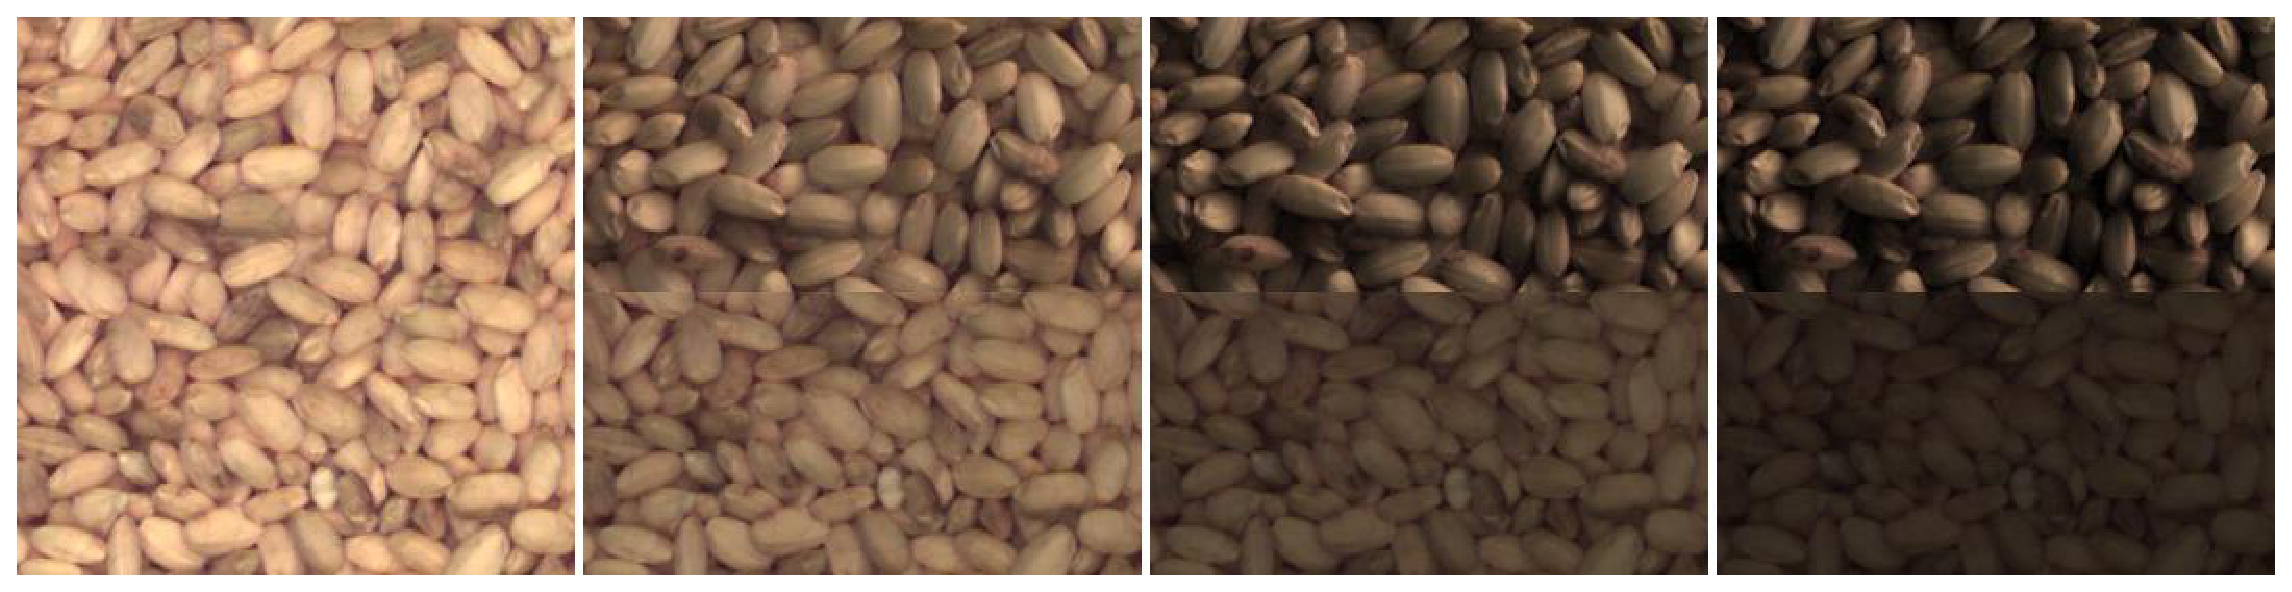
\includegraphics[scale=.4]{image_eps/ptm/ptm.eps}
% \label{fig:subfig3} } \caption{PTM vs Conventional Texture Map: The upper portions of the images shows the visual appearance of
% a PTM while the bottom half shows the conventional Texture map. Note how the former appears realistic while
% the later suffers from unrealistic lighting and shadows.
% } \label{fig:subfigureExample}
% \end{figure*}
% \end{center}
% The reflectance function of a scene point captures the appearance of that
% point as a function of lighting direction. We present an approach to printing
% the reflectance functions of an object or scene so that its appearance is
% modified correctly as a function of the lighting conditions when viewing the
% print. For example, such a “photograph�? of a statue printed with our approach
% appears to cast shadows to the right when the “photograph�? is illuminated
% from the left. Viewing the same print with lighting from the right will cause
% the statue’s shadows to be cast to the left. Beyond shadows, all effects
% due to the lighting variation, such as Lambertian shading, specularity, and
% inter-reflection can be reproduced. We achieve this ability by geometrically
% and photometrically controlling specular highlights on the surface of the
% print. For a particular viewpoint, arbitrary reflectance functions can be built
% up at each pixel by controlling only the specular highlights and avoiding
% significant diffuse reflections. Our initial binary prototype uses halftoning
% to approximate continuous grayscale reflectance functions.
% 
% An object’s appearance changes when lit from different directions.
% Shadows are cast and specular highlights shine. Even diffuse sur-
% faces change appearance, providing a valuable perceptual cue to ob-
% ject shape and material. Unfortunately, when printed on paper, this
% variability is lost. A photographic print represents just one appear-
% ance, regardless of the ambient lighting when the print is viewed.
% A real scene’s appearance at each point depends upon the in-
% cident illumination, the surface Bi-directional Reflectance Distri-
% bution Function (BRDF) [Nicodemus et al. 1977], and the local
% surface orientation. Typical printers cannot print images which re-
% act to incident illumination because they use inks with a limited
% range of BRDFs and print on paper which is flat, having a single
% orientation everywhere.
% Simply expanding the range of specularity of the printer’s inks is
% insufficient. Surface orientation plays an important role in control-
% ling the observed intensity of reflected light. To correctly represent
% this interaction with light, the local surface orientation of the paper
% needs to match that of the original object.
% A conceptually simple solution would be to orient the local sur-
% face normal of each pixel appropriately, and to print the object’s
% surface BRDF onto this pixel. However, this requires changing the
% physical shape of the underlying paper at the time of printing. This
% is an expensive process that requires equipment far more complex
% than just depositing ink onto a surface.
% We introduce a method of printing reflectance functions [Debevec
% et al. 2000] which makes use of paper with a static microgeometry
% structure, shown in Figure 1(b). The paper consists of a hexago-
% nal array of spherical depressions that have a specularly reflective
% surface. By selectively printing opaque or partially opaque ink on
% portions of that surface, we can control whether a specific inci-
% dent lighting direction returns a specular highlight, and to what
% degree. Because both the paper and ink are designed to minimize
% diffuse reflections, the specular return fully controls the appearance
% of this “reflectance paper�? and is used to control its appearance as a
% function of lighting direction. Note that this scheme gives sufficient
% expressive power to specify two dimensions of the 4D BRDF. We
% choose to specify, for a single fixed viewing direction, how much
% light will be reflected from each incident lighting direction, thereby
% building up an arbitrary reflectance function.
% The primary contribution of this work is a method for printing
% reflectance functions using existing printers and special paper. We
% support this contribution with a ray traced simulation and analysis
% of errors, as well as with an initial prototype implementation.
% 
% D reflectance functions can be measured easily for real scenes
% by taking photographs lit from many different lighting directions,
% and a wide variety of devices have been constructed to do so
% [Debevec et al. 2000; Malzbender et al. 2001; Peers et al. 2006;
% Wenger et al. 2005]. In principle this function can contain
% high-frequency components from specular highlights and hard
% shadows. However, in practice even low-order approximations are
% sufficient for a variety of presentation and evaluation purposes
% [Hawkins et al. 2001; Ramamoorthi et al. 2001]. Manipulations
% of reflectance functions have proved useful especially in both
% cinema applications [Debevec et al. 2000; Peers et al. 2007] and
% archeological applications [Freeth et al. 2006; Mudge et al. 2006].
% Figure 2 shows several examples of reflectance functions for in-
% dividual pixels, parameterized by the incoming illumination angle.
% 
% On the left is a set of colored leaves, with the reflectance of spe-
% cific marked pixels shown below. On the right are pixels chosen on
% opposite edges of almonds. Note that shadows are present in both
% cases at extreme lighting angles, and this shows up as dark regions
% in the reflectance function. Although the reflectance functions are
% very smooth, they are oriented differently at different pixels, and
% this is sufficient to provide a convincing perception of object shape
% when the incident light angle is changed. Flat paper printed with
% standard inks can only represent centered isotropic functions similar
% to the red pixel in this example. Our design can represent arbitrary
% functions. Note that for the photographically collected reflectance
% functions we employ, global illumination effects such as shadows
% and interreflections are present at the time of image capture, and thus
% are represented in the reflectance function. Whether such secondary
% effects are modeled is dependent on the generation of the reflectance
% data that is input to our system, whether captured or simulated.


\section{Polynomial Texture Maping}
To be written.
% PTM Representation
% Instead of representing light-dependent texture maps as a large number of source images, a compact 
% representation that can be rapidly evaluated is necessary. The representation used in Polynomial Texture Maps is 
% especially well suited for real-time games. For most materials other than mirrored surfaces the reflected light 
% varies smoothly as a function of incident light direction. This is because materials with rough microstructures 
% scatter light across a range of directions rather than a single reflected direction. As a result, in the illuminant
% domain the reflected light can be reproduced with low frequency representations. Any high-frequency effects that 
% do exist are blurred in light space and become smoother. Shadows cast by point light sources result in high 
% frequency changes in light space. Modeling with low frequency representations simply softens the hard shadows
% into what would be caused by area light sources. None of the softening in light space results in perceptually
% objectionable changes as it results in a plausible rendered appearance. Figure 2 shows two examples of PTMs 
% rendered from different illumination directions.
% The representation used in Polynomial Texture Maps is a biquadratic polynomial, which has sufficient degrees of 
% freedom to represent many different types of materials and objects while requiring a small number of parameters 
% per texel. The function used in PTMs is:
% 
% L(u,v;l ,l ) a (u,v)l a (u,v)l a (u,v)l l a (u,v)l a (u,v)l a (u,v) u v u v 2 u v 3 u 4 v 5
% 
% The lu and lv input values are the projection of the desired incident light direction onto the tangent and binormal in 
% the local texture coordinate system. The tangent and binormal are calculated as in other tangent space shading 
% methods based on the geometry and texture coordinates. The PTM representation has six coefficients a0..a5 that 
% are fit to the captured source images for every texel. Six scale and bias values are stored for each PTM to allow 
% the calculated coefficients to be stored at 8-bit precision while reproducing the range parameters. Typical 
% materials do not change their color significantly when the illumination direction is changed. For those materials, a 
% single polynomial per texel can be used to represent the texel luminance function. A separate normalized RGB 
% 
% One of the advantages of this polynomial representation is that the output luminance depends linearly on the PTM 
% coefficients. This linearity means that applying mip-mapping and texture filtering directly on the coefficients 
% results in the correct appearance from the filtered coefficients. This is an improvement over bump mapping 
% techniques where naively filtering the bump map results in smoothing of the bump surface and incorrect 
% renderings. 
% When a luminance polynomial and RGB image is used for light-dependent texture mapping the storage 
% requirements are 6 8-bit coefficients and 3 8-bit color values per texel. While this is more data than standard 
% texture maps, this is much less data than the original source images that the PTMs reproduce. Compression 
% algorithms can be used to further reduce the size of the PTM. If compression is needed for offline storage than a 
% variant of JPEG can be used. By using JPEG compression on planes of coefficients for some of the coefficients, 
% and predicting other planes from the intracoded planes significant compression can be achieved with little 
% perceptual artifacts. For compression that can be processed by the GPU other techniques can be investigated. For
% example, vector quantization can be implemented directly on the GPU and should achieve good compression for 
% PTM datasets.
% The PTM technique is also useful for modeling other appearance effects that map well onto the polynomial 
% representation. For example, focus variation can be captured from photographs of a scene at multiple focus
% depths. The polynomial per texel then models the appearance of a pixel as a function of focal depth rather than
% light direction. The polynomial function can be reduced to a simpler 1D function as necessary depending on the 
% number of degrees of freedom. Other simple 1D and 2D effects that can be modeled with the low-frequency 
% representation can also be reproduced. High-frequency lighting such as specular highlights can also be rendered 
% by combining PTMs with existing rendering techniques. Most synthetic lighting models require the surface 
% normal for rendering. It is simple to estimate the surface normal for every texel of a PTM representing a diffuse 
% object. Since diffuse objects are brightest when the incident light direction aligns with the surface normal we can 
% solve for the light direction that maximizes the polynomial function to estimate the normal. During rendering the 
% PTM is evaluated as usual to recreate the captured material and then combined with the synthetic specular 
% reflectance.
% 
% Polynomial Texture Maps is a pixel based technique used to model luminiance
% against changing lighting direction.PTMs reconstruct the color of a surface under varying lighting
% conditions. When a surface is rendered with a PTM, it takes on different illumination
% characteristics depending on the direction of the light source.
% (uncommented)
% 
% PTM model uses a set of input images captured from a fixed camera, where each
% image is illuminated from a specific known lighting direction. It uses a
% biquadratic polynomial function with 6 coefficients per pixel for modeling the
% reflectance. These coefficients are estimated from the set of input images(30 to
% 40), where the lighting direction is resolved into two components i.e
% $l_{u}$,$l_{v}$ by projecting it on the image plane. These two components are
% used as variables in the biquadratic function. Once the coefficients are
% estimated fitting the model to the observed values, they are used to render
% images from any given lighting direction.
% 
% 
% 
% In a typical setup, a camera is mounted
% at the apex of a hemisphere of lights, and each light is then fired in turn, thus generating a
% sequence of images. Usually, some 40 to 50 images are used, with the larger the number of
% images the better.
% Thus PTM is a pixel-based method for modelling dependency of luminance (or RGB in a
% different embodiment) on lighting with the objective being relightable images. At each pixel,
% a 6-vector of coefficients is calculated using nonlinear least squares over the 2-vector of light-
% ing direction x, y-projected components. Subsequently, re-rendering can take place, e.g. by
% relighting images using a new lighting direction, by calculating surface normals and thence
% generating artificial specular highlights, by re-mapping colour, by increasing directional sen-
% sitivity to lighting direction in order to enhance contrast, by light source extrapolation, or by
% artificially varying focus
% 
% Polynomial Texture Mapping enables greatly improved realism
% over conventional methods. Traditional texture mapping is used to
% give the impression of geometric detail in a model using an image.
% For example, a photograph of a brick wall may be used as a
% texture map on a planar surface to avoid modeling the complex
% surface detail of the brick. However, if the lighting in the
% synthetic environment where the texture map is used is different
% from the lighting the texture map was captured under, the
% resulting rendering will appear incorrect and unrealistic. Worse
% yet, when the texture is blended with the calculated lighting of a
% geometric surface, the resulting rendering will look very flat and
% smooth to the viewer.
% 
% Bump mapping [Blinn 78] is one proposed solution to this
% problem where the surface normals of underlying geometry are
% allowed to vary per texture element (texel). Introducing variations
% in the surface normals causes the lighting method to render the
% surface as though it had local surface variations instead of just a
% smooth surface. As a result, when the light is moved around the
% object, highlights appear due to the bump map and the surface
% appears to be rough, grooved or similarly modified as desired.
% Bump maps can be either hand modeled or, more typically,
% calculated procedurally. Creating a bump map to be used with real
% world textures from photographs is generally difficult. Methods
% have been developed that attempt to automatically generate bump
% maps from a set of input images under known light directions
% [Rushmeier 97]. These methods have difficulty with generating
% bump maps for objects with large surface variations that cause
% self-shadowing and intra-object interreflections. In addition,
% current bump map rendering techniques do not render shadows
% due to surface variation or brightened regions due to
% interreflections.
% 
% In contrast, our method is an image-based technique that requires
% no modeling of complex geometry or bump maps. The input data
% required is a set of images of the desired object to be used as a
% texture, each one under illumination from a different known
% direction, all captured from the same view point. The input light
% irections need not be uniformly spaced in the hemispherical set
% of possible light directions. We choose to represent the variation
% in surface color for each pixel independently with a simple
% biquadratic
% polynomial.
% Although
% approximate,
% this
% representation is compact and allows fast color reconstruction
% during rendering. One implementation of our method uses a
% polynomial to approximate the luminance of each texel, keeping
% the chromaticity constant. The result of our method is a texture
% map that properly reproduces the effects of variations in the
% illuminant direction relative to the object, whether due to the
% surface orientation of the texture-mapped object, or to changing of
% the location of the source. Intensity and color variations that are
% also due to self shadowing, sub-surface scattering and
% interreflections are also captured and modeled by PTMs. Figure 1
% compares our method to conventional texture mapping as lighting
% varies. Renderings using our method are very realistic, and require
% little or no user input once the input images are acquired.

% The PTM technique causes overall smoothening of light which dampens the effect
% of specularity and softens sharp shadows. The effect of point light source is
% reduced and the appearance is always similar to a diffused light source. Towards
% this end, Drew {\em et al.} proposed modeling of shadows and
% highlights in addition the the basic matt texture. The goal of this approach is
% specifically to interpolate between two given images, and not a 3D texture model
% of the surface.
% 
% We improve upon the PTM model to overcome the above limitations
% and generate a complete 3D Texture model that can be evaluated at individual
% pixels. We propose an approach to image-based lighting interpolation that is
% based on estimates of geometry and shading from a set of input images. We
% decompose images captured at different lighting conditions into intrinsic image
% components; i.e, the {\em direct} and {\em global} image components. Each of
% these components is then further separated to obtain different physical
% phenomena such as shadows, specularity and luminance. A final image is obtained
% by combining the the individual models together.